\documentclass[9pt,twocolumn,twoside,]{pnas-new}

%% Some pieces required from the pandoc template
\providecommand{\tightlist}{%
  \setlength{\itemsep}{0pt}\setlength{\parskip}{0pt}}

% Use the lineno option to display guide line numbers if required.
% Note that the use of elements such as single-column equations
% may affect the guide line number alignment.

%%
%%


%%
%%

\usepackage[T1]{fontenc}
\usepackage[utf8]{inputenc}

% Pandoc citation processing
\newlength{\csllabelwidth}
\setlength{\csllabelwidth}{3em}
\newlength{\cslhangindent}
\setlength{\cslhangindent}{1.5em}
% for Pandoc 2.8 to 2.10.1
\newenvironment{cslreferences}%
  {}%
  {\par}
% For Pandoc 2.11+
\newenvironment{CSLReferences}[3] % #1 hanging-ident, #2 entry spacing
 {% don't indent paragraphs
  \setlength{\parindent}{0pt}
  % turn on hanging indent if param 1 is 1
  \ifodd #1 \everypar{\setlength{\hangindent}{\cslhangindent}}\ignorespaces\fi
  % set entry spacing
  \ifnum #2 > 0
  \setlength{\parskip}{#2\baselineskip}
  \fi
 }%
 {}
\usepackage{calc} % for calculating minipage widths
\newcommand{\CSLBlock}[1]{#1\hfill\break}
\newcommand{\CSLLeftMargin}[1]{\parbox[t]{\csllabelwidth}{#1}}
\newcommand{\CSLRightInline}[1]{\parbox[t]{\linewidth - \csllabelwidth}{#1}}
\newcommand{\CSLIndent}[1]{\hspace{\cslhangindent}#1}


\templatetype{pnasresearcharticle}  % Choose template

\title{Modelling a primate technological niche}

\author[a]{Jonathan S Reeves}
\author[a]{Tomos Proffitt}
\author[a]{Lydia Luncz}

  \affil[a]{Max Planck Institute for Evolutionary Anthropology,
Technological Primate Research Group, Deutscher Platz 6., Leipzig,
Germany, 04103}


% Please give the surname of the lead author for the running footer
\leadauthor{Reeves}

% Please add here a significance statement to explain the relevance of your work
\significancestatement{Primate tool-use is generally considered to be
expedient and largely restricted to places where tool materials and
resources occur in close proximity. Our model shows how the repeated
transport of stone tools over short distances can expand where tool-use
can occur beyond the natural landscape. These results demonstrate the
capacity for chimpanzee technological behavior to modify environments
over time. However, inferring this behavior from its material record may
prove difficult given mismatches between the behavior and its
archaeological signature.}


\authorcontributions{Please provide details of author contributions
here.}

\authordeclaration{There are no conflicts of interest.}


\correspondingauthor{\textsuperscript{2} E-mail:
\href{mailto:jonathan_reeves@eva.mpg.de}{\nolinkurl{jonathan\_reeves@eva.mpg.de}}}

% Keywords are not mandatory, but authors are strongly encouraged to provide them. If provided, please include two to five keywords, separated by the pipe symbol, e.g:
 \keywords{  Tool Transport |  Niche Construction |  Percussive
tools |  Primate Archaeology |  Agent-Based Modeling  } 

\begin{abstract}
Tool transport has been fundamental to the success of our lineage. The
relocation of materials from where they naturally occur to where they
are needed modifies the environment in a way that increases access to a
broader landscape. In contrast, transport of tools over long distances
has never been observed in primates. However, chimpanzee stone tools
have been recorded farther from their raw material source than what is
expected from ethological observations. The mechanisms through which the
long distance relocation of tool material occurs is currently unknown.
Here we present an agent-based model, built on observations of wild
chimpanzee tool transport, that explores the relationship between
tool-use, the environment, and the formation of the archaeological
record. While our results show that primate tool-use is largely
constrained by the environment, there are circumstances in which the
aggregated effect of small-scale tool transport can dramatically
increase the distribution of tool material across a wider landscape over
time. This highlights the capacity for small-scale transport to
increases the accessibility of otherwise inaccessible resources over
time. Moreover, understanding the landscape patterning that this
behavior produces will help us to draw corollaries between tool behavior
and its archaeological record. While our results also suggest that these
processes leave tangible traces in the archaeological record, they are
variable and alerts us to the disparity between observed behaviors and
their archaeological signature.
\end{abstract}

\dates{This manuscript was compiled on \today}
\doi{\url{www.pnas.org/cgi/doi/10.1073/pnas.XXXXXXXXXX}}

\begin{document}

% Optional adjustment to line up main text (after abstract) of first page with line numbers, when using both lineno and twocolumn options.
% You should only change this length when you've finalised the article contents.
\verticaladjustment{-2pt}

\maketitle
\thispagestyle{firststyle}
\ifthenelse{\boolean{shortarticle}}{\ifthenelse{\boolean{singlecolumn}}{\abscontentformatted}{\abscontent}}{}

% If your first paragraph (i.e. with the \dropcap) contains a list environment (quote, quotation, theorem, definition, enumerate, itemize...), the line after the list may have some extra indentation. If this is the case, add \parshape=0 to the end of the list environment.

\acknow{We thank the Max Planck Society for supporting this research. We
also thank the Max Planck Institute for Evolutionary Anthropology for
hosting our research group. JSR thanks the Luke Premo for providing
feedback and thoughtful discussion on an earlier version of this work.}

The adaptive success of humans is largely based on the transport of
tools to overcome environmental constraints. Over human evolutionary
history, this trait has facilitated the expansion of humans and their
ancestors across every environment in the terrestrial world (1). The
onset of long distance transport in the Early Stone Age initiated the
wider access to resources, allowing hominins to exploit a broader
landscape (2). This ability to modify the broader environment through
the use and relocation of tool material is considered to be a hallmark
of the human niche (3, 4). In contrast, stone tool transport in
non-human primates is considered to be generally constrained by the
environment as tool use only happens when tool materials and food
resources occur in the same location and only transport over short
distances has been observed (5, 6). In the Tai Forest, Côte d'Ivoire,
chimpanzee stone hammers have been recorded kilometers from their
nearest raw material source (7). However, it is not known whether this
form of transport constitutes a modification of the environment that
subsequently influences behaviors. Understanding the mechanisms by which
chimpanzees move tools over long distances is important as it
redistributes tool material. This, in turn, may influence tool-using
opportunities providing access to resources across a broader landscape
(5).

Moreover, there is a growing consensus that primate like tool-use may
have been the precursor to the current earliest physical evidence of
tool-use and transport in the archaeological record of hominins (8).
However, there is little understanding of what this record may look like
(but see (8)). Thus, understanding the broader dynamics of primate
tool-use may help develop expectations for the archaeological signature
of the early tool use hominins.

Understanding how individual bouts of small scale tool-use produce
landscape scale patterning and subsequently the formation of the
archaeological record requires bridging multiple temporal gaps (9).
Daily observations of extant primate stone tool use reflect individual
behavior, whereas their landscape scale material record likely
represents the aggregation of many tool-using events of over multiple
years (7). Furthermore, the earliest archaeological record often
reflects hundreds if not thousands of years of time (10). As a result,
neither the development of landscape wide patterns of wild primate
tool-use nor the subsequent formation of the archaeological record can
be directly observed.

Behavioral processes such as transport, re-use, and use-life are known
to have a substantial influence on the patterning of the archaeological
record (11). This is particularly pertinent to primate tool-use as some
groups repeatedly re-use the same tools over time (12). The dynamic
movement and reuse of stone tools over time is argued to lead an
underrepresentation of percussive technology in the chimpanzee
archaeological record (13). Despite the fact that Chimpanzees were
frequently observed to crack nuts with large stone hammers, no complete
hammerstones were recovered from archaeological contexts (13).
Therefore, understanding the relationship between primate tool-use, the
broader landscape, and its archaeological corollaries requires methods
that examine the development of patterns across multiple temporal
scales.

Here we present an agent-based model (ABM) that is designed to bridge
the gaps between the various temporal disconnects between individual
behaviors, environmental process, and the formation of the
archaeological record. To investigate the effect of primate tool-use on
the broader distribution of tool materials, we model small scale tool
transport and use, akin to chimpanzee nut-cracking. We varied the number
of resources -- sources of stone and tool-use locations - to further
understand the environmental circumstances in which the movement of
tools over long distances occur. In doing so, we are also able to
examine the effect of tool transport on the future opportunities for
tool-use and the accessibility of resources over time as well as how
such dynamics structure the formation of the archaeological record.

\hypertarget{materials-and-methods}{%
\section{Materials and Methods}\label{materials-and-methods}}

The model was designed and implemented using Python 3 and the ABM
library Mesa (14). The model consists of a 250 x 250 grid-cell space
that is populated with four types of agents; \emph{Primates},
\emph{Sources}, \emph{Trees}, and \emph{Pounding Tools}. This grid space
can be thought of as a forest in which agents move across the landscape,
transporting stone tools over small distances as they encounter
resources that require tool use to access. The tool-use behavior
implemented in the model, is designed to approximate Panda nut cracking
of Western Chimpanzees (15). \emph{Primates} are agents that can be
thought of as chimpanzees who move around the landscape cracking nuts at
any opportunity. \emph{Sources} are stationary agents whose locations
reflect places where \emph{Pounding Tools} can be acquired
(e.g.~inselburgs and cobble beds). \emph{Sources} can vary in their
``quality'' which determines how likely \emph{Pounding Tools} are to
break and lose mass during use.

\emph{Pounding Tools} are analogous to the hammers used to crack nuts.
\emph{Pounding Tools} vary in their mass (grams) and ``quality.'' The
size of the Pounding Tool is determined by randomly drawing from a
normal distribution with mean and standard distribution equivalent to
the mass of the stone hammers recovered in the Tai Forest (7). Quality
refers to the likelihood a tool will break during use and subsequently
lose mass and is determined by the ``quality'' of the \emph{Source} it
is acquired from. \emph{Pounding Tools} can be continuously re-used
until they break so much that they are too small (less than 2000 grams)
to be used as tools. This size threshold is equivalent to a small Panda
nut cracking hammer in the Tai Forest (7).

\emph{Trees} are agents that represent locations where tool use can
occur. While \emph{Trees} exist only at fixed locations, the death and
regrowth of trees within a forest can restructure where the resources
are accessible over time (8). To simulate this process, \emph{Trees}
increase in age by a unit of 1 after each time-step and will die when
their age is equal to 10,000 time steps. When a \emph{Tree's} age
reaches 10,000 time-steps nut-cracking can no longer take place at its
location and a new location within a 10 grid-cell radius is randomly
chosen as a place for a new \emph{Tree} to ``grow.'' Though the death
and growth of \emph{Trees} are not linked in this way in the natural
world, this ensures that the number of \emph{Trees} remains constant
during the simulation.

When the model is initialized, \emph{Trees}, \emph{Sources}, and
\emph{Primates} are randomly placed within the grid-cell space. Each
\emph{Source} is randomly assigned an integer of 0, 25, 50, or 75
representing raw material quality. To prevent every \emph{Tree} from
dying at the same time-step, each \emph{Tree} is randomly assigned an
age between 1 and 10000. \emph{Trees} that grow after model initialized
begin with an age 0. The population of \emph{Primates} was held constant
at 100 for each run of the model. The number of \emph{Sources} range
between 10, 100, 500. The number of \emph{Trees} varied between 100,
500, 1000, or 2000. The duration of each model run was 75,000 time
steps.

During each time-step, \emph{Primates} move a length of 1 grid-cell in a
random direction. If the \emph{Primate} moves into a grid-cell that
neighbors or is occupied by a \emph{Tree}, the \emph{Primate} will check
to see if a \emph{Source} or \emph{Pounding Tool} is within a radius 2
grid-cells around its location. If there is none, then the
\emph{Primate} continues to move. If a \emph{Source} is within the
search radius of the \emph{Primate}, then the \emph{Primate} will
acquire a \emph{Pounding Tool} from this location. If a previously used
\emph{Pounding Tool} is found within the search area, then the
\emph{Primate} will re-use the \emph{Pounding Tool}. In the event that
both \emph{Sources} and \emph{Pounding Tools} are found within the
search radius then the \emph{Primate} will choose the \emph{Pounding
Tool} or \emph{Source} that is nearest to its location. If multiple
\emph{Pounding Tools} or \emph{Sources} are equally near, then the
choice is random.

To simulate small scale tool transport and use, the \emph{Primate} moves
the acquired \emph{Pounding Tool} to the location of the \emph{Tree} or
one of its neighboring grid-cells where it is used and discarded. The
likelihood that a \emph{Pounding Tool} will break is determined by a
baseline probability of 25\% plus its fragility. For example, if the
fragility of the raw material is 25, this is added to the baseline
making the break probability for this tool 50\%. When a \emph{Pounding
Tool} breaks, an additional \emph{Pounding Tool}, classified as a
fragment, is discarded at the location. The size of the resulting
``fragment'' is modeled after the observed size distribution of
fragments detached from \emph{Pounding Tools} during modern and ancient
chimpanzee nut-cracking events in which most breakages result in the
production of small fragments but in rare cases fragments can also be
large (13).

During the simulation, the model records data about the broader
environment as well as each individual \emph{Pounding Tool}. At the
global level, the model monitors proximity of live \emph{Trees} to
unexhausted \emph{Pounding Tools} and \emph{Sources}. In iterations
where \emph{Trees} can die and grow the model also keeps track of the
location of the \emph{Trees} as they change through time. In addition,
each \emph{Pounding Tool} records the \emph{Source} that it originated
from, the number of times it was used for nut-cracking, its initial size
and its size after use as well as its location at the end the
simulation. At the end of the simulation the model outputs the location
of each \emph{Pounding Tool} and any discarded fragments,
\emph{Sources}, and \emph{Trees} as well as their attributes. This
provides a means to examine the relationship between where tool-use
occurs and the location of \emph{Sources} and \emph{Trees} from both
systemic and archaeological perspectives.

\hypertarget{results}{%
\section{Results}\label{results}}

\hypertarget{environment-tool-use-dynamics}{%
\subsubsection{Environment-Tool Use
Dynamics}\label{environment-tool-use-dynamics}}

\begin{figure}
\centering
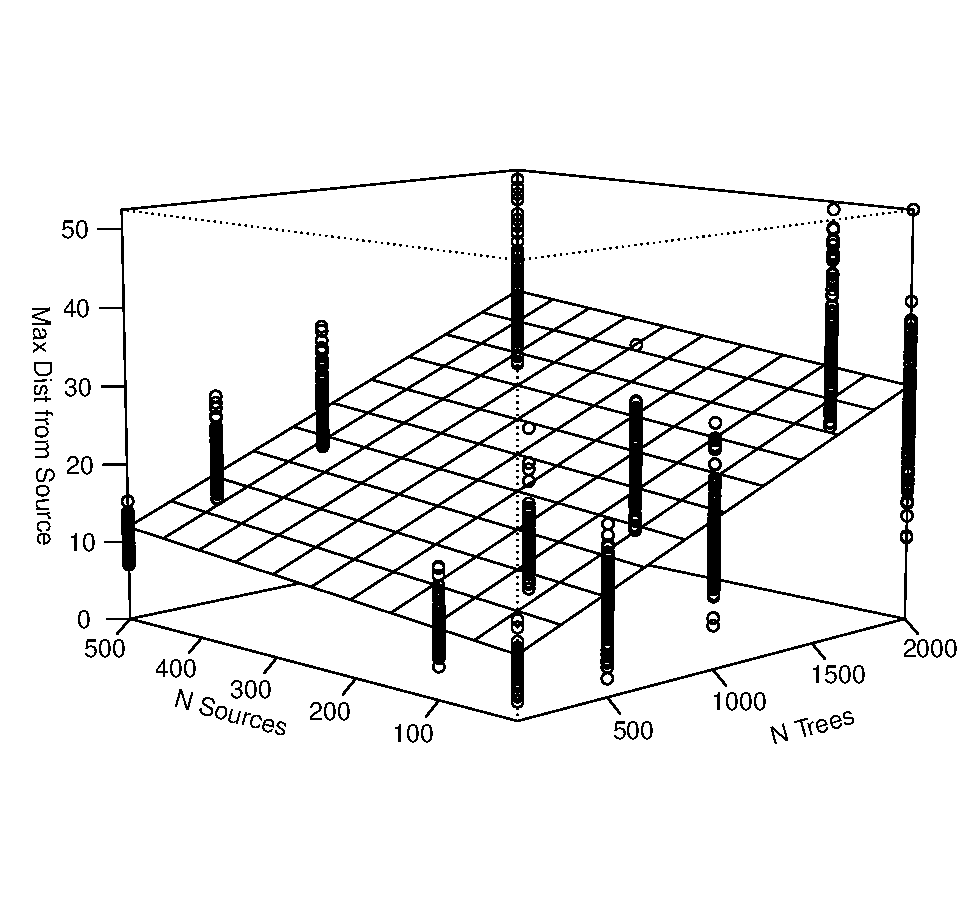
\includegraphics{Reeves_et_al_2021_Panda_ABM_files/figure-latex/figure 1-1.pdf}
\caption{A two-way interaction plots illustrating the effect of the
number of \emph{Trees} and number of \emph{Sources} on distance maximum
distance \emph{Pounding Tools} move from its source. The number of
sources has a marginal effect on the maximum distances \emph{Pounding
Tools} move in the model whereas, increasing the number of \emph{Trees}
has a dramatic effect. \label{d2source}}
\end{figure}

At the beginning of each model run tool-use can only occur in places
where a \emph{Tree} is a maximum distance of 3 grid cells from a
\emph{Source}. Simply increasing both the number of \emph{Sources}
and/or \emph{Trees} increases the number of places where tool-use is
possible (SOM Figure 1: left, ANOVA, F: 2435.41, P-value: 0). Tool-use
occurred at \emph{Trees} located more than 3 grid cells from the nearest
source in 95\% of the runs. When a \emph{Pounding Tool} is moved from a
\emph{Source}, it becomes a secondary source of material for other
\emph{Trees}. Provided \emph{Trees} are within three grid cells, tools
can be moved between them. As a result, repeated small scale transport
can incrementally move \emph{Pounding Tools} up to a maximum distance of
58 grid cells from their original \emph{Sources}. Consequently, this
redistribution of tools increases the number of opportunities for
tool-use across a wider landscape. At the end of 88\% of all runs, there
are more places where tool-use can occur than at the beginning (Figure
\ref{d2source}). The runs that did not show an increase in tool-use
opportunities are those where the number of \emph{Trees} are initially
low (SOM Table 3).

The results of the model show how opportunities for tool-use are
impacted by the structure of the environment. \emph{Pounding Tools} move
greater maximum distances when the number of \emph{Trees} increases
(Figure \ref{d2source}, left). The frequency that \emph{Pounding Tools}
can be transported and used is regulated by their size and quality.
However, the relatively small size of detached fragments allows Pounding
Tools to be utilized 35s to 400s of times prior to exhaustion. While
higher quality materials move greater maximum distances (SOM Figure:
XX), the potentially long use-life of \emph{Pounding Tools} result in a
similar spatial distribution regardless of quality.

The interplay between changing \emph{Tree} locations and the extended
use-life of \emph{Pounding Tools} further facilitates the incremental
distribution of tool materials across the landscape. When the numbers of
\emph{Sources} and \emph{Trees} are held constant, iterations where
\emph{Trees} change their location (i.e life-cycle) increases the
distance \emph{Pounding Tools} can move. When \emph{Tree} locations
remains static, the number of opportunities for tool use, over time,
eventually plateaus and no more loci become available (Figure
\ref{tree_death}, top). Conversely, when \emph{Tree} locations are
dynamic, opportunities for tool use does not plateau or diminish over
time. Instead, the number of Trees where tool use is possible continues
to increase (Figure \ref{tree_death}, right) despite the fact that
\emph{Pounding Tool} transport and \emph{Tree} life cycles operate on
different temporal scales.

\begin{figure*}

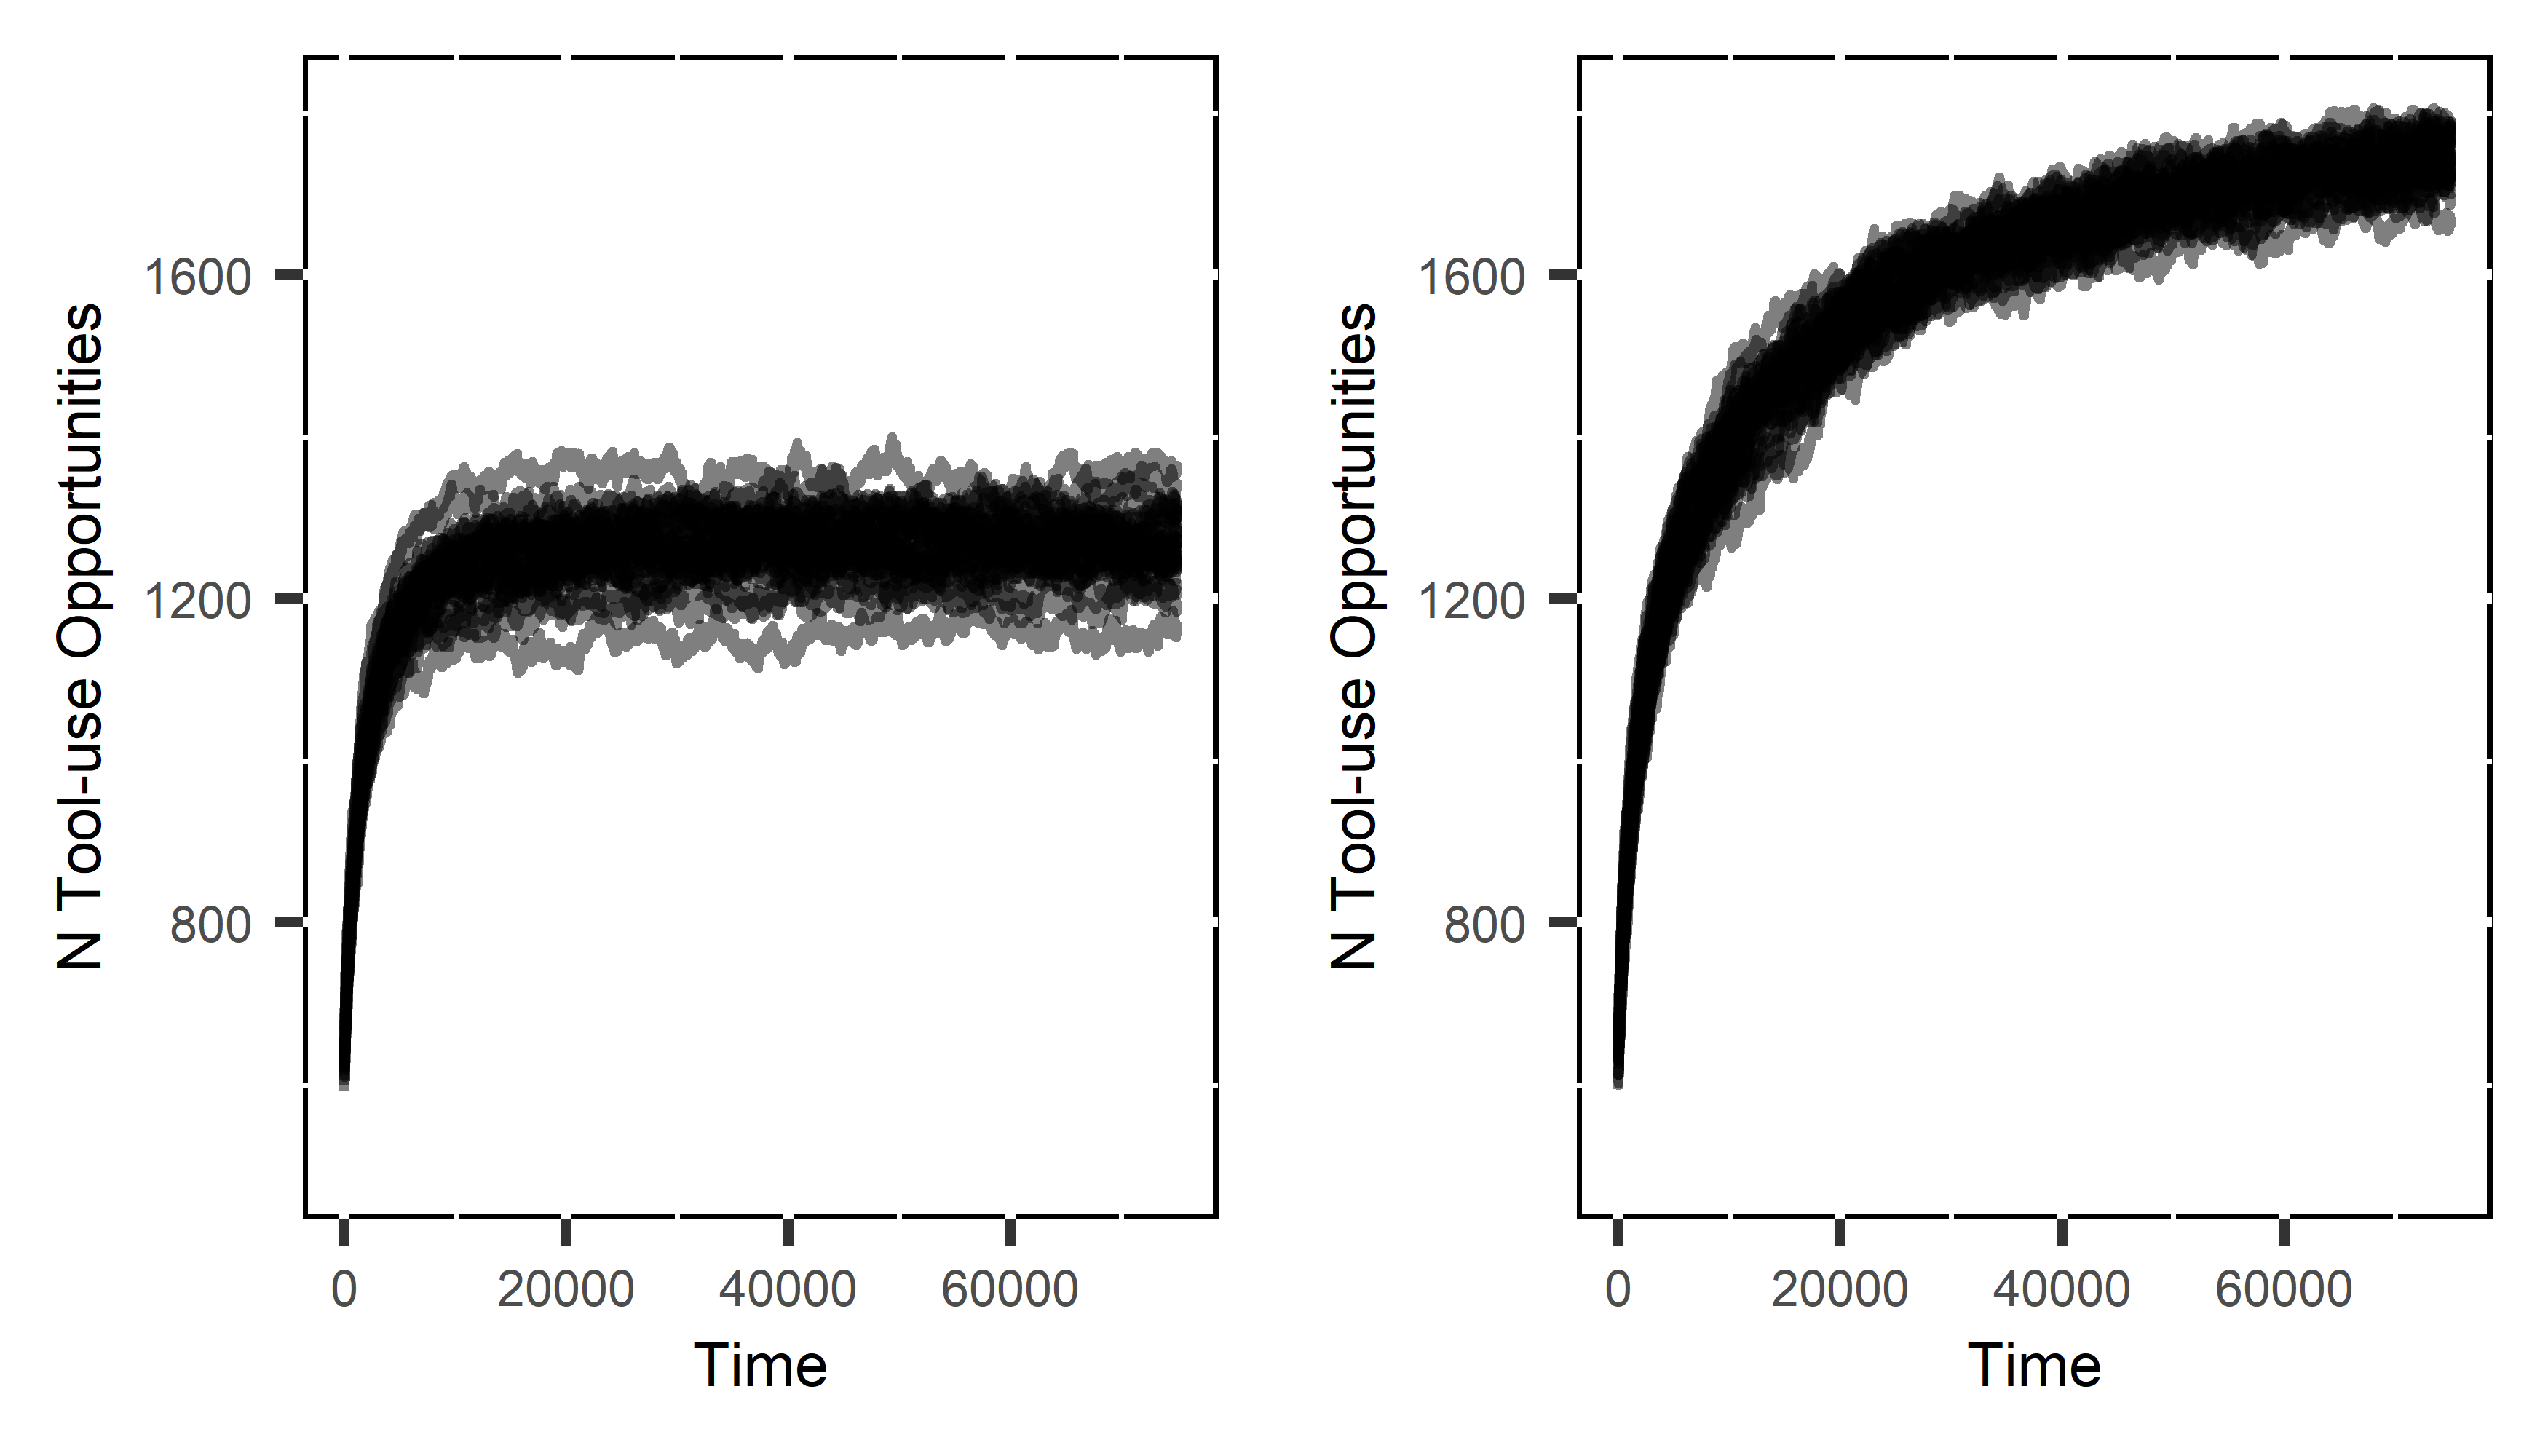
\includegraphics[width=6.5in]{Reeves_et_al_2021_Panda_ABM_files/figure-latex/figure 2-1.png}

\caption{Time series plots illustrating the changes in the number of tool use locations over time when Trees are static (Top) and when they are dynamic (Bottom) for runs where the number of soures is 500 and the number of trees is 2000. The ticks on the y-axes of the color plots to the left represent individual interations of the model. The X-axis represents the time step in the model run. Therefore, any individual cell of color represents the number of locations where tool-use is possible. Each line in the plots to the right represents an individual itetation of model with time represented on the x-axis and the number of tool-use locations is represented on the y-axis. Note that in iterations where tree locations is dynamic the number of tool-use locations is always greater. The slope of the lines (right) show that the number of tool-using locations will continue to increase instead of plateauing.}

\label{tree_death}

\end{figure*}

\hypertarget{material-signature}{%
\subsubsection{Material Signature}\label{material-signature}}

The modeled behavior creates a material record that is comprised
predominantly of fragments detached from \emph{Pounding Tools}, but also
exhausted and functional Pounding Tools in substantially smaller
quantities. The spatial distribution, density and composition of the
material record is dependent on the environmental circumstances that
facilitate the movement of \emph{Pounding Tools}. When \emph{Trees} are
infrequent, the resulting assemblages form localized patches in the
grid-cells nearest to \emph{Sources} (Figure \ref{distribution}, left).
As the number of Trees increases, the material record becomes more
wide-spread (Figure \ref{distribution}, middle). \emph{Tree} life cycles
have the greatest effect on the distribution of the archaeological
record across space (Figure \ref{distribution}, right). These results
show that small scale transport, tool-use, coupled with varying resource
densities and environmental stability can substantially influence the
structure of the archaeological record.

\begin{figure*}

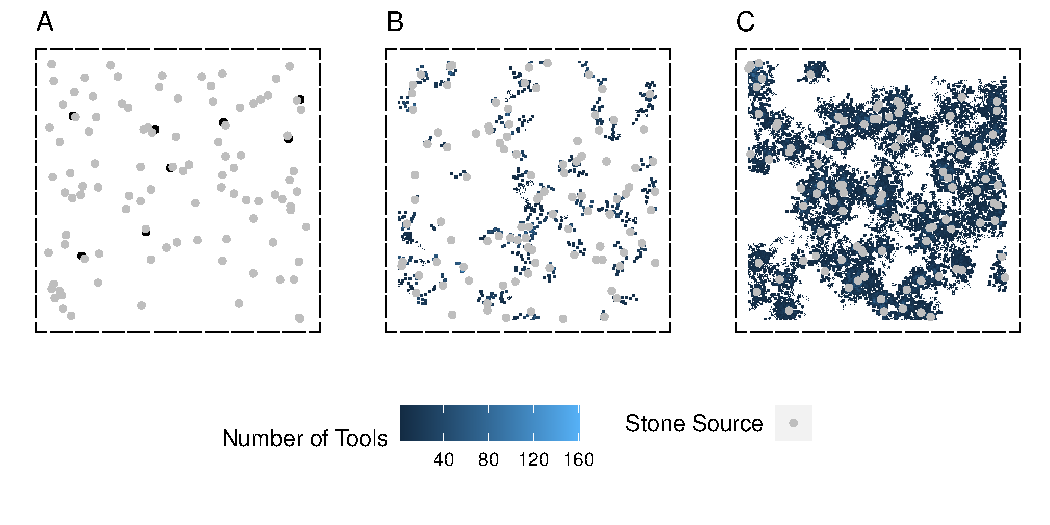
\includegraphics[width=6.5in]{Reeves_et_al_2021_Panda_ABM_files/figure-latex/figure 3-1.pdf}

\caption{A: The archaeological record when there are 100 sources and 100 trees. Notice that the subsequent archaeological record forms extremely localized patches of material. B: The archaeological record there 100 sources and 2000 trees. This archaeological record is becoming more wide-spread but remains localized. C: The archaeological record there 100 sources and 2000 trees where trees can die and regrow. The notice how the the growth and death of trees becomes substantially more widespread.}

\label{distribution}

\end{figure*}

The total amount of discarded material per grid cell, the number of
\emph{Pounding Tools} and the mass of \emph{Pounding Tools} form a
distance-decay pattern in which these variables are negatively
correlated with the distance to Source locations (Figures
\ref{assemblages}, SOM Figure 5). The wide range of variance in these
metrics in locations closer to \emph{Sources} is also due to the local
configuration of Trees. If the location of Trees does not facilitate
\emph{Pounding Tool} movement then the associated will only occur within
the grid cells closest to the Sources (Figures \ref{assemblages}, SOM
Fig. 6, SOM Fig. 7). It is important to note that while this behavior
can produce a widespread material record, \emph{Pounding Tools} are not
found in every grid-cell that accumulates an assemblage. Environmental
circumstances that promote the movement of \emph{Pounding Tools} across
space (i.e numbers of \emph{Trees} or dynamic \emph{Tree} locations)
have a negative effect on the proportion of grid-cells that contain
re-usable tools (Figure \ref{pounding_tools}). In cases, where tools can
move large distances, assemblages with \emph{Pounding Tools} comprise as
little as 2.5\% of the broader material record. This suggests there
maybe some material records where usable \emph{Pounding Tools} are not
easily recovered.

\hypertarget{discussion}{%
\section{Discussion}\label{discussion}}

The model illustrates the dynamic relationship between small scale
tool-use and transport, the environment, and the formation of the
archaeological record. Agents only engaged in tool use during chance
encounters where tool material could be moved short distances to tool
using locations. Though these results show that resources ultimately
dictate the opportunities for tool use, in some circumstances, the
aggregate effect of this behavior led to the widespread redistribution
of tool material across the landscape. Repeated small scale tool
transport has the power to move beyond the constraints of the natural
environment to increase the number of opportunities for tool use at
future time-steps. Moreover, this process can work in tandem with the
changing distribution of tool use localities over time to further
increase the spread of tool material across the landscape. As a result,
the landscape that agents inhabit at time step 0 is different to the one
they inhabit at time step 75000.

\begin{figure*}

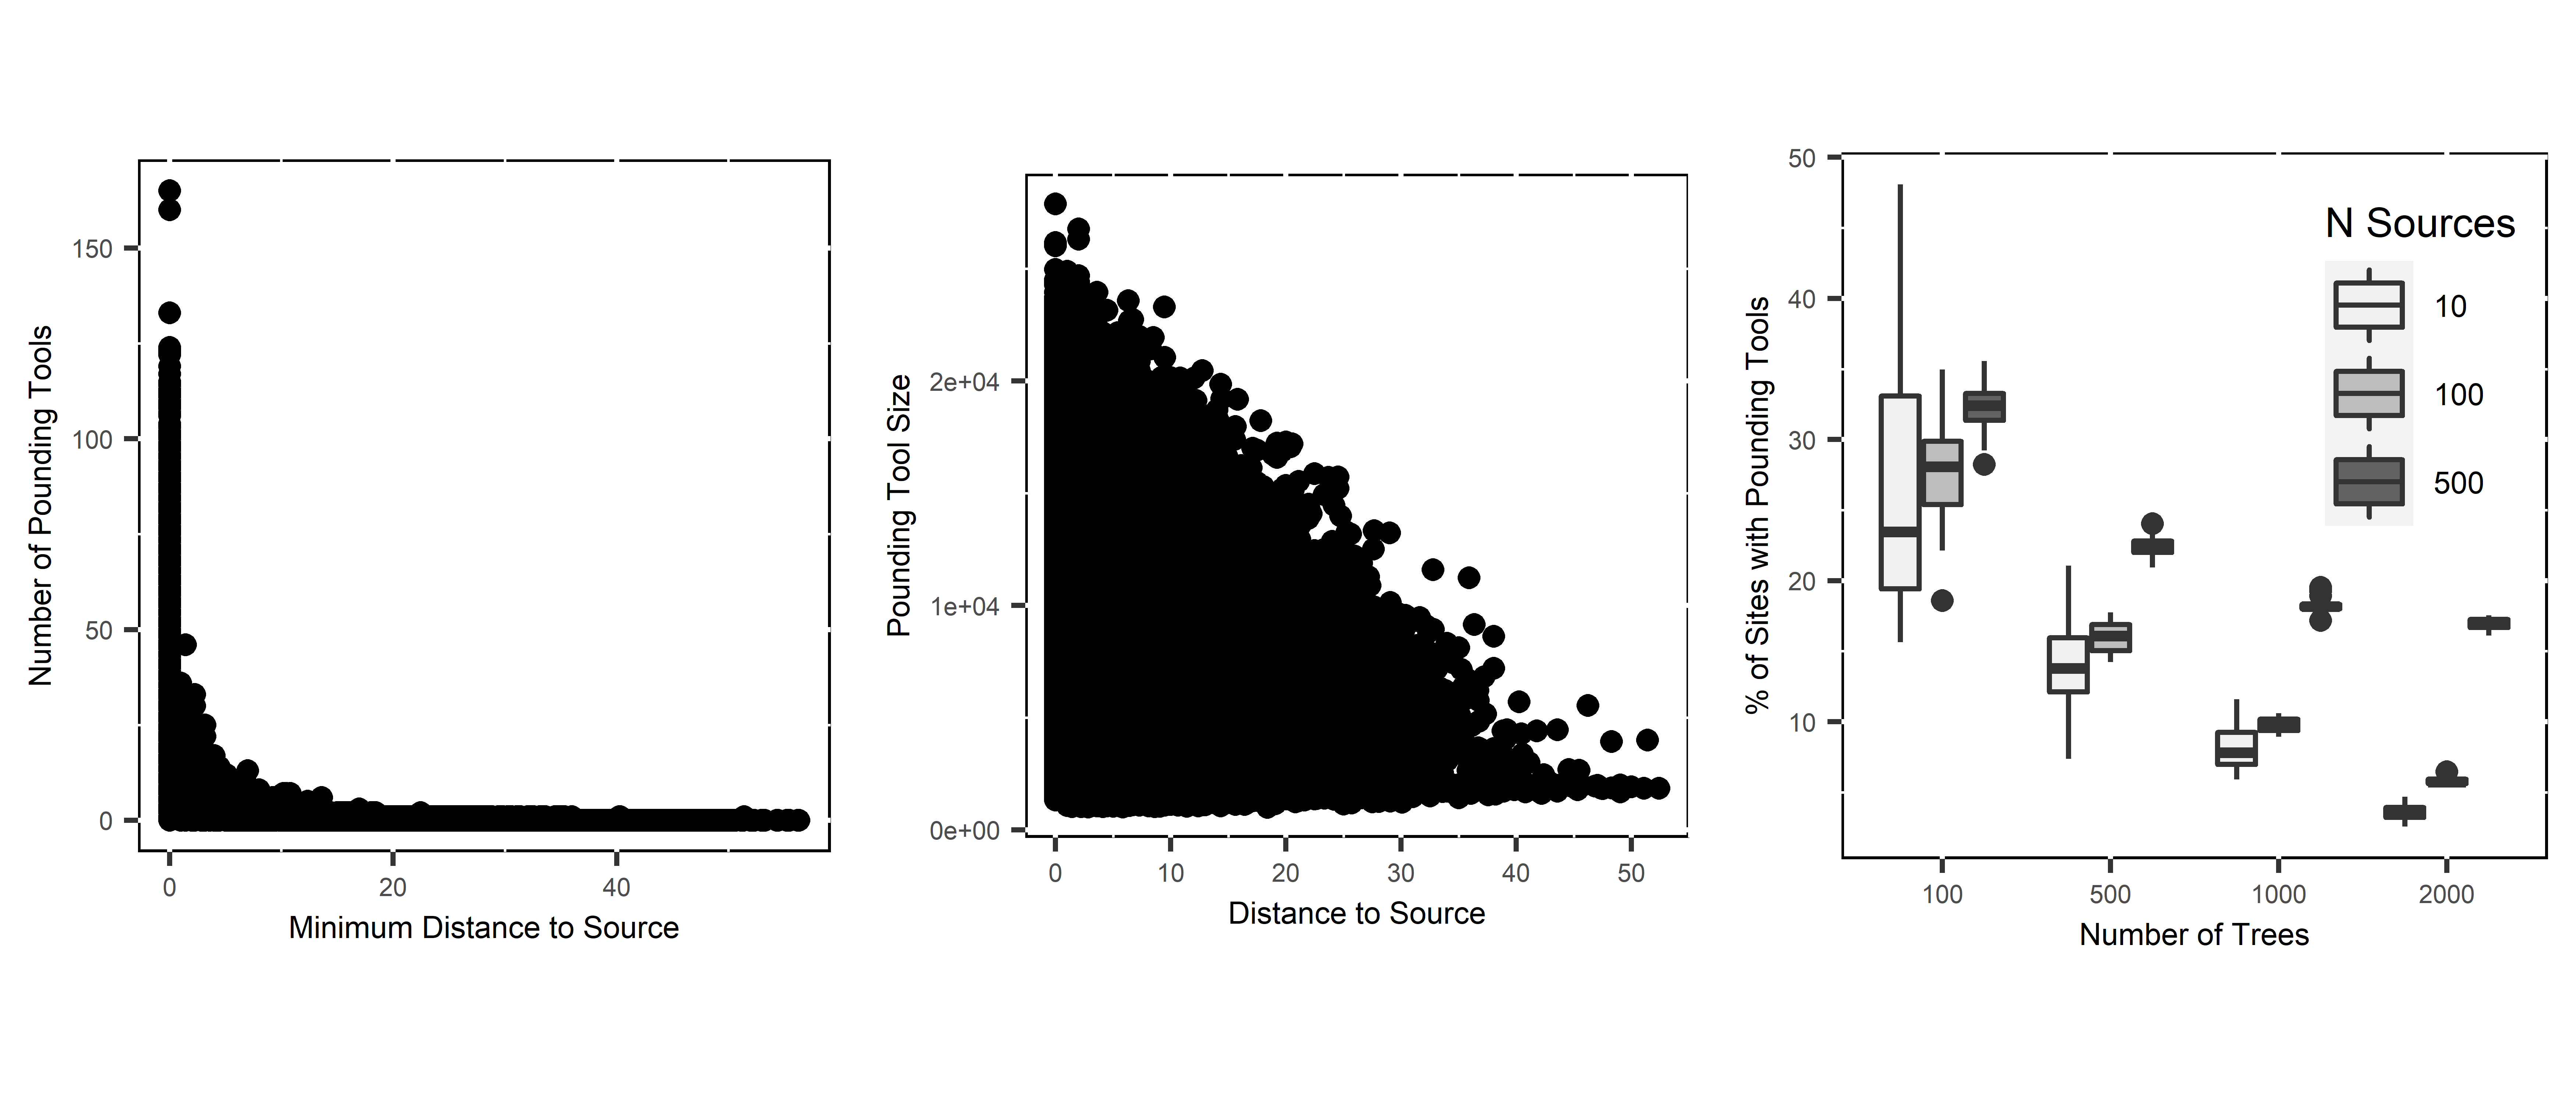
\includegraphics[width=6.5in]{Reeves_et_al_2021_Panda_ABM_files/figure-latex/figure 4-1.png}

\caption{Left: A scatter plot showing the relationship between the number of artifacts (e.g. Pounding Tools and fragments) present within a grid-cell and its distance to the nearest source. Grid-cells closer to sources can possess a wider range of artifacts, whereas grid-cells farther from the source consistently possess few artifacts. Middle: Scatter plot showing the relationship of the number Pounding Tools in a grid cell with the distance to the nearest source. Right: The relationship between Pounding Tool size and distance to its source. Note: All plots show runs where the number of sources is 100 and the number of trees is 2000. See SOM figures 5, 6, and 7 for other model runs.}

\label{assemblages}

\end{figure*}

Within primate populations, it has been argued that patterns of tool
assisted foraging are largely constrained by encounter rates with
resources (5, 16). It has been suggested that long distance movements of
tools must occur on rare occasions (17) or that the repeat short term
transport of tools can result the movement of tools over long distances
(McGrew 1992). This, however, has never been observed (7). Here, our
model shows that single long distance tool transport events are not
needed to distribute percussive tools across the wider landscape. The
aggregate effect of this behavior can increase the number of tool use
opportunities over time and space. This illustrates the niche
constructing capacity of primate tool using behaviors. The widespread
distribution of pounding tools facilitated by their long use-lives
generates feedback in which future generations inherit a landscape where
opportunities for tool use are greater than they were before. More
opportunities for tool-use increases the potential for the acquisition
of tool using skills {[}(5); (6); {]}. Therefore, small scale tool
transport produces a landscape which may ensure the continuation of tool
behaviors across generations.

\begin{figure}
\centering
\includegraphics{Reeves_et_al_2021_Panda_ABM_files/figure-latex/figure 5-1.pdf}
\caption{The effect of the environment on the representation of
\emph{Pounding tools} in the simulated material record. Increasing the
number of sources increases the percentage of assemblages that contain
\emph{Pounding Tools}. Increasing the number of \emph{Trees} or allowing
the \emph{Tree} locations to be dynamic substantially reduces the
proportion of assemblages that contain useable tools
\label{pounding_tools}}
\end{figure}

In this light, the results of the model provide a context for exploring
how primates modify their landscape beyond the scope of ethological
observations. In the Tai Forest, hammerstones have been recorded up to 2
kilometers from the nearest raw material source (7). Furthermore, the
distribution of the size and wear of these hammerstones is consistent
with the distance-decay relationship described in the model (7).
Although short distance transport of tools is observed in the Tai
Forest, the broader spatial distribution is the end product of
individual behaviors that remain undetected as they mostly happen in the
absence of observers. This model illustrates the mechanism by which
chimpanzees of the Tai Forest could emergently modify the distribution
of tool materials across space through repeated re-use and transport of
hammerstones. This may imply that, given that tool use is considered to
be socially learned (18), chimpanzees may increase their accessibility
to resources through a culturally learned behavior.

The interaction between tool transport and the modeled environmental
change could be applied to any resource that change location over time.
Beyond the implications for living primates, the model also illustrates
how processes that operate on different temporal scales can interact to
increase opportunities for tool use. In hominin evolutionary studies,
one of the challenges of understanding the relationship between hominins
and their environments through time is the need to link small scale
behavioral processes with long term ecological dynamics (9, 19, 20). Few
mechanisms that causally link local scale environmental change to
behavior have, however, been purposed or identified (21). Though the
behavior of the agents in our model does not change over time, our model
illustrate how processes that operate on different temporal scales
(i.e.~tool use life and environmental stability) can work in tandem to
produce feedback that enhances opportunities for the behavior across
space and time. Feedback loops such as the one described here may have
influenced opportunities and access of resources to hominins prior to
the advent of intentional long distance transport.

The results of the model provide novel insights into the translation of
dynamic behavior into the static archaeological record. The material
records generated by the undirected forging strategies of the agents
range from localized patches to structured distance decay-patterns. Both
of these spatial patterns have been argued as evidence of intentional
behavior reflecting planning, foresight, and land use strategies in the
hominin record (22, 23). Yet, we show that it is possible to produce
both by solely varying the spatial distribution of resources without
changing behavior. Our results emphasize the importance of the interplay
between the environment and behavior in structuring the archaeological
record (8, 24). In the case of our model, a widespread material record
can emerge as a consequence of the interaction between small scale tool
transport, tool re-use, use-life, and resource distributions over time.
Understanding the mechanisms by which tools are moved and discarded
become increasingly critical for interpreting the patterns described in
the archaeological record.

\hypertarget{conclusion}{%
\section{Conclusion}\label{conclusion}}

Though small scale tool-use is ultimately constrained by its
environment. This model shows that hammerstone transport over time can
have a significant effect on the facilitation of tool behavior itself.
The aggregate effect of short transportation events can improve the
accessibility of resources within a landscape over time. This landscape
pattern of unintentional tool provisioning not only potentially
mitigates against local changes in the availability of resources but
also increases the opportunity for nut cracking to be carried out. In
this sense this tool-using behavior provides chimpanzees and potentially
other tool-using non-human primates the capacity to positively modify
their environments.. In the context of living Chimpanzee populations,
the results of the model in combination with ethological data have the
potential to incrementally modify their environments through a
culturally learned behaviors.

In sum, small scale tool transport is ultimately constrained by the
environment. However, our model illustrates how aggregate effect of
short transportation events increases the accessibility of resources
across a wider landscape over time. Furthermore, these results show that
the modeled behavior can also interact with changes in landscape
structure that further promote increases in the tool-use opportunities.
This highlights the capacity for tool transport to emergently modify
their environments over the long-term, thus, enhancing the technological
niche across generations.

\showmatmethods
\showacknow
\pnasbreak

\hypertarget{references}{%
\section*{References}\label{references}}
\addcontentsline{toc}{section}{References}

\hypertarget{refs}{}
\begin{CSLReferences}{0}{0}
\leavevmode\hypertarget{ref-hillEmergenceHumanUniqueness2009}{}%
\CSLLeftMargin{1. }
\CSLRightInline{Hill K, Barton M, Magdalena Hurtado A (2009) The
emergence of human uniqueness: {Characters} underlying behavioral
modernity. \emph{Evolutionary Anthropology} 18(5):187--200.}

\leavevmode\hypertarget{ref-pottsWhyOldowanPlioPleistocene1991}{}%
\CSLLeftMargin{2. }
\CSLRightInline{Potts R (1991) Why the {Oldowan}? {Plio}-{Pleistocene
Toolmaking} and the {Transport} of {Resources}. \emph{Journal of
Anthropological Research} 47(2):153--176.}

\leavevmode\hypertarget{ref-lalandNicheConstructionBiological2000}{}%
\CSLLeftMargin{3. }
\CSLRightInline{Laland KN, Odling-Smee J, Feldman MW (2000) Niche
construction, biological evolution, and cultural change.
\emph{Behavioral and Brain Sciences} 23(1):131--146.}

\leavevmode\hypertarget{ref-haasForagerMobilityConstructed2019}{}%
\CSLLeftMargin{4. }
\CSLRightInline{Haas R, Kuhn SL (2019) Forager {Mobility} in
{Constructed Environments}. \emph{Current Anthropology} 60(4):499--535.}

\leavevmode\hypertarget{ref-koopsEcologyCultureEnvironmental2013}{}%
\CSLLeftMargin{5. }
\CSLRightInline{Koops K, McGrew WC, Matsuzawa T (2013) Ecology of
culture: Do environmental factors influence foraging tool use in wild
chimpanzees, {Pan} troglodytes verus? \emph{Animal Behaviour}
85(1):175--185.}

\leavevmode\hypertarget{ref-visalberghiDistributionPotentialSuitable2009}{}%
\CSLLeftMargin{6. }
\CSLRightInline{Visalberghi E, et al. (2009) Distribution of potential
suitable hammers and transport of hammer tools and nuts by wild capuchin
monkeys. \emph{Primates} 50(2):95--104.}

\leavevmode\hypertarget{ref-lunczDistancedecayEffectStone2016}{}%
\CSLLeftMargin{7. }
\CSLRightInline{Luncz LV, Proffitt T, Kulik L, Haslam M, Wittig RM
(2016) Distance-decay effect in stone tool transport by wild
chimpanzees. \emph{Proceedings of the Royal Society B: Biological
Sciences} 283(1845):20161607.}

\leavevmode\hypertarget{ref-pangerOlderOldowanRethinking2003}{}%
\CSLLeftMargin{8. }
\CSLRightInline{Panger MA, Brooks AS, Richmond BG, Wood B (2003) Older
than the {Oldowan}? {Rethinking} the emergence of hominin tool use.
\emph{Evolutionary Anthropology: Issues, News, and Reviews}
11(6):235--245.}

\leavevmode\hypertarget{ref-stinerChallengesDocumentingCoevolution2020}{}%
\CSLLeftMargin{9. }
\CSLRightInline{Stiner MC (2020) The challenges of documenting
coevolution and niche construction: {The} example of domestic spaces.
\emph{Evolutionary Anthropology}:evan.21878.}

\leavevmode\hypertarget{ref-sternImplicationsTimeaveragingReconstructing1994}{}%
\CSLLeftMargin{10. }
\CSLRightInline{Stern N (1994) The implications of time-averaging for
reconstructing the land-use patterns of early tool-using hominids.
\emph{Journal of Human Evolution} 27(1-3):89--105.}

\leavevmode\hypertarget{ref-schifferFormationProcessesArchaeological1987}{}%
\CSLLeftMargin{11. }
\CSLRightInline{Schiffer MB (1987) \emph{Formation processes of the
archaeological record} ({University of New Mexico Press}) Available at:
\url{https://books.google.co.ke/books/about/Formation_processes_of_the_archaeologica.html?id=TMpVlJ8zK78C\&redir_esc=y}.}

\leavevmode\hypertarget{ref-boeschMentalMapWild1984}{}%
\CSLLeftMargin{12. }
\CSLRightInline{Boesch C, Boesch H (1984) Mental map in wild
chimpanzees: {An} analysis of hammer transports for nut cracking.
\emph{Primates} 25(2):160--170.}

\leavevmode\hypertarget{ref-proffittRevisitingPanda1002018}{}%
\CSLLeftMargin{13. }
\CSLRightInline{Proffitt T, Haslam M, Mercader JF, Boesch C, Luncz LV
(2018) Revisiting {Panda} 100, the first archaeological chimpanzee
nut-cracking site. \emph{Journal of Human Evolution} 124:117--139.}

\leavevmode\hypertarget{ref-masadMESAAgentBasedModeling2015}{}%
\CSLLeftMargin{14. }
\CSLRightInline{Masad D, Kazil J (2015) {MESA}: {An Agent}-{Based
Modeling Framework}. \emph{Proceedings of the 14th Python in Science
Conference (SCIPY 2015)}:53--60.}

\leavevmode\hypertarget{ref-boeschWildCulturesComparison2014}{}%
\CSLLeftMargin{15. }
\CSLRightInline{Boesch C (2014) \emph{Wild cultures a comparison between
chimpanzee and human cultures.} ({Cambridge University Press},
{Cambridge}).}

\leavevmode\hypertarget{ref-carvalhoToolcompositeReuseWild2009}{}%
\CSLLeftMargin{16. }
\CSLRightInline{Carvalho S, Biro D, McGrew WC, Matsuzawa T (2009)
Tool-composite reuse in wild chimpanzees ({Pan} troglodytes):
Archaeologically invisible steps in the technological evolution of early
hominins? \emph{Anim Cogn} 12(1):103--114.}

\leavevmode\hypertarget{ref-whitenArchaeologyMeetsPrimate2013}{}%
\CSLLeftMargin{17. }
\CSLRightInline{Whiten A (2013) Archaeology meets primate technology.
\emph{Nature} 498(7454):303--305.}

\leavevmode\hypertarget{ref-whitenCulturesChimpanzees1999}{}%
\CSLLeftMargin{18. }
\CSLRightInline{Whiten A, et al. (1999) Cultures in chimpanzees.
\emph{Nature} 399(6737):682--685.}

\leavevmode\hypertarget{ref-iovitaOperationalizingNicheConstruction2021}{}%
\CSLLeftMargin{19. }
\CSLRightInline{Iovita R, et al. (2021) Operationalizing niche
construction theory with stone tools. \emph{Evolutionary
Anthropology}:evan.21881.}

\leavevmode\hypertarget{ref-kingstonShiftingAdaptiveLandscapes2007}{}%
\CSLLeftMargin{20. }
\CSLRightInline{Kingston JD (2007) Shifting {Adaptive Landscapes}:
{Progress} and {Challenges} in {Reconstructing Early Hominid
Environments}. \emph{Yearbook of Physical Anthropology} 50:20--58.}

\leavevmode\hypertarget{ref-behrensmeyerClimateChangeHuman2006}{}%
\CSLLeftMargin{21. }
\CSLRightInline{Behrensmeyer AK (2006) Climate {Change} and {Human
Evolution}. \emph{Science} 311(5760):476--478.}

\leavevmode\hypertarget{ref-plummerFlakedStonesOld2004}{}%
\CSLLeftMargin{22. }
\CSLRightInline{Plummer TW (2004) Flaked stones and old bones:
{Biological} and cultural evolution at the dawn of technology.
\emph{Yearbook of Physical Anthropology} 47:118--164.}

\leavevmode\hypertarget{ref-blumenschineEffectsDistanceStone2008}{}%
\CSLLeftMargin{23. }
\CSLRightInline{Blumenschine RJ, Masao FT, Tactikos JC, Ebert JI (2008)
Effects of distance from stone source on landscape-scale variation in
{Oldowan} artifact assemblages in the {Paleo}-{Olduvai Basin},
{Tanzania}. \emph{Journal of Archaeological Science} 35(1):76--86.}

\leavevmode\hypertarget{ref-brooksPreservationActivityAreas1987}{}%
\CSLLeftMargin{24. }
\CSLRightInline{Brooks AS, Yellen JE (1987) The {Preservation} of
{Activity Areas} in the {Archaeological Record}: {Ethnoarchaeological}
and {Archaeological Work} in {NOrthwest Ngamiland}, {Botswana}.
\emph{Methog and {Theory} for {Activity Area Research}: {An
Ethnoarchaeological Approach}} ({Columbia University Press}, {New
York}), pp 63--106.}

\end{CSLReferences}



% Bibliography
% \bibliography{pnas-sample}

\end{document}
